\documentclass[11pt]{article}
% DEFINE COMMANDS

\usepackage{NotesTeX}

\usepackage[font=small,labelfont=bf]{caption}
\usepackage{enumerate}
\usepackage{amsmath,amssymb,amscd,amsfonts}
\usepackage{xcolor}
\usepackage{color}
\input{undertilde}


\usepackage{tikz}
\usepackage{tikz-cd}
\tikzcdset{every label/.append style = {font = \small}}
\tikzcdset{row sep/normal=3.5em}
\tikzcdset{column sep/normal=3.5em}

\usetikzlibrary{matrix}
\usetikzlibrary{decorations.markings,calc,shapes}
\usetikzlibrary{positioning}
\usepackage{graphicx}
\usepackage{empheq}
\usepackage{physics}
\usepackage{siunitx}
\usepackage{tensor}

\usepackage{multicol}

\usepackage{youngtab}
\usepackage{cancel}
\usepackage{caption}
\usepackage{graphicx}
\usepackage{subcaption}
\usepackage{hyperref}

\usepackage{float}
% added by Jingtian Shi
\usepackage{indentfirst}
\usepackage{cases}
\usepackage{bbm}
\usepackage{slashed}
\newcommand{\rqm}{{\declareslashed{}{\text{-}}{0.04}{0}{I}\slashed{I}}}

\makeatletter
\RenewDocumentCommand\sidenotetext{ o o +m }{%
    \IfNoValueOrEmptyTF{#1}{%
        \@sidenotes@placemarginal{#2}{\textsuperscript{\thesidenote}{}~\footnotesize#3}%
        \refstepcounter{sidenote}%
    }{%
        \@sidenotes@placemarginal{#2}{\textsuperscript{#1}~#3}%
    }%
}
\makeatother
% % % % % % % % % % % % % % % % % % % % % % %

\title{{\Huge General Relativity}\\{\Large{Class 40 --- May 1, 2020}}} %replace with class number
\author{Irakli Jokhadze}

\emailAdd{ijokhadze@utexas.edu} %replace with your email
\begin{document}
\maketitle
\flushbottom
\newpage
\pagestyle{fancynotes}



\section{Energy of Gravitational waves}
Last time we introduced a stress energy tensor that represents energy content of gravitational waves (GWs). The problem is that it is not gauge invariant.
This problem was solved by Isacson (1968) who led out the formalism to solve this problem: short-wavelength approximation (two length scale approximation).

Suppose there is some curved spacetime background and on that curved spacetime background we have GWs with relatively high frequencies - we have two scales in problem.
There is one scale L long distance over which the background spacetime has some kind of curvature $L \sim 1/\sqrt{R}$ which is infinite for the flat spacetime.
The second scale corresponds to the wavelength $\lambda$ of the radiation.  
 



    \begin{figure} [H]
        \begin{center}









\tikzset{every picture/.style={line width=0.75pt}} %set default line width to 0.75pt

\begin{tikzpicture}[x=0.75pt,y=0.75pt,yscale=-1,xscale=1]
%uncomment if require: \path (0,300); %set diagram left start at 0, and has height of 300

%Curve Lines [id:da8918658251950633]
\draw    (225.04,164.2) .. controls (245.48,107.61) and (258.88,99.34) .. (270.39,110.66) .. controls (296.7,136.56) and (313.13,264.91) .. (381.27,152.2) ;
%Shape: Free Drawing [id:dp4500985972474567]
\draw  [color={rgb, 255:red, 0; green, 0; blue, 0 }  ][line width=0.75] [line join = round][line cap = round] (15.7,169.2) .. controls (21.35,169.2) and (13.9,155.24) .. (16.35,149.2) .. controls (18.37,144.21) and (19.94,155.68) .. (20.23,156.4) .. controls (20.33,156.64) and (20.24,157.47) .. (20.23,157.2) .. controls (19.99,151.07) and (16.72,143.14) .. (20.23,138.8) .. controls (21.97,136.65) and (23.67,143.28) .. (24.77,146) .. controls (25.29,147.28) and (25.93,151.43) .. (26.06,150) .. controls (26.63,143.63) and (23.04,126.27) .. (26.71,130.8) .. controls (28.02,132.42) and (29.01,134.42) .. (29.95,136.4) .. controls (30.53,137.64) and (31.14,141.83) .. (31.24,140.4) .. controls (31.79,132.96) and (25.84,118) .. (31.89,118) .. controls (34.79,118) and (33.09,126.27) .. (35.78,127.6) .. controls (37.58,128.49) and (35.65,122.79) .. (35.78,120.4) .. controls (35.85,118.96) and (35.96,112.18) .. (37.07,110.8) .. controls (39.77,107.47) and (42.52,120.1) .. (43.55,122) .. controls (43.79,122.44) and (43.46,120.92) .. (43.55,120.4) .. controls (43.9,118.24) and (44.28,116.09) .. (44.84,114) .. controls (45.58,111.28) and (46.3,108.51) .. (47.43,106) .. controls (49.13,102.23) and (49.98,114.02) .. (51.32,118) .. controls (51.58,118.78) and (51.78,116.41) .. (51.97,115.6) .. controls (53.1,110.7) and (51.7,109.53) .. (55.2,105.2) .. controls (57.18,102.76) and (57.62,115.38) .. (59.09,117.2) .. controls (60.66,119.14) and (60.15,110.54) .. (62.33,110) .. controls (67.14,108.81) and (65.51,119.31) .. (66.21,122.8) .. controls (66.84,125.92) and (70.57,112.55) .. (71.39,115.6) .. controls (73.45,123.23) and (68.95,131.58) .. (69.45,139.6) .. controls (69.65,142.85) and (73.87,128.35) .. (73.98,131.6) .. controls (74.2,137.99) and (74.19,144.41) .. (73.98,150.8) .. controls (73.97,151.18) and (73.16,151.91) .. (73.34,151.6) .. controls (81.77,136.72) and (79.07,143.32) .. (79.81,158) .. controls (79.94,160.45) and (81.81,151.62) .. (83.7,152.4) .. controls (87.07,153.79) and (81.21,177.32) .. (86.94,165.2) .. controls (87.87,163.23) and (87.86,160.7) .. (88.88,158.8) .. controls (89.15,158.3) and (89.51,159.8) .. (89.53,160.4) .. controls (89.73,167.33) and (88.87,174.31) .. (89.53,181.2) .. controls (90.04,186.56) and (89.87,169.45) .. (92.77,171.6) .. controls (96.51,174.37) and (94.04,182.27) .. (94.71,187.6) .. controls (94.81,188.43) and (95.4,180.4) .. (99.24,180.4) .. controls (101.98,180.4) and (101.17,193.06) .. (101.18,193.2) .. controls (101.21,193.53) and (105.12,184.83) .. (107.01,186) .. controls (110.82,188.35) and (109.16,201.2) .. (111.55,201.2) .. controls (115.25,201.2) and (113.84,189.63) .. (116.08,192.4) .. controls (118.69,195.62) and (117.92,200.15) .. (119.32,203.6) .. controls (119.84,204.88) and (120.01,200.83) .. (120.61,199.6) .. controls (121.57,197.63) and (122.54,195.62) .. (123.85,194) .. controls (126.23,191.05) and (127.94,200.65) .. (130.33,203.6) .. controls (130.76,204.13) and (131.31,202.65) .. (131.62,202) .. controls (132.65,199.88) and (133.63,196.32) .. (134.86,194.8) .. controls (136.03,193.35) and (139.36,200.58) .. (139.39,200.4) .. controls (140.12,195.62) and (138.55,189.44) .. (141.34,186) .. controls (143.04,183.89) and (144.1,196.92) .. (144.57,194) .. controls (145.07,190.92) and (143.39,182.44) .. (145.87,180.4) .. controls (147.67,178.92) and (147.82,185.61) .. (149.75,186.8) .. controls (150.72,187.4) and (149.57,184.11) .. (149.75,182.8) .. controls (150.3,178.98) and (150.12,174.35) .. (152.34,171.6) .. controls (153.79,169.82) and (154.4,175.95) .. (155.58,178) .. controls (156.22,179.11) and (156.04,175.34) .. (156.23,174) .. controls (156.73,170.5) and (156.89,166.78) .. (158.17,163.6) .. controls (159.04,161.45) and (165.2,172.52) .. (165.3,172.4) .. controls (166.58,170.81) and (164.7,161.97) .. (167.24,160.4) .. controls (170.34,158.48) and (169.32,171.92) .. (172.42,170) .. controls (175.32,168.21) and (172.31,161.95) .. (171.77,158) .. controls (171.61,156.82) and (171.16,160.36) .. (170.48,161.2) ;
%Shape: Free Drawing [id:dp5077635597975942]
\draw  [color={rgb, 255:red, 0; green, 0; blue, 0 }  ][line width=0.75] [line join = round][line cap = round] (421.47,157) .. controls (421.63,156.55) and (424.7,147.46) .. (424.79,148.2) .. controls (425.17,151.38) and (424.88,154.9) .. (425.74,157.8) .. controls (425.9,158.33) and (426.02,156.7) .. (426.21,156.2) .. controls (427.07,154.03) and (427.91,146.37) .. (429.53,148.2) .. controls (429.88,148.59) and (431.23,158.14) .. (431.43,157.8) .. controls (432.46,156.05) and (431.55,148.86) .. (432.85,147.4) .. controls (434.93,145.06) and (435.92,154.1) .. (437.11,157.8) .. controls (437.55,159.16) and (440.41,142.63) .. (441.85,146.6) .. controls (443.01,149.76) and (443.18,153.73) .. (444.22,157) .. controls (444.91,159.15) and (446.72,146.8) .. (448.49,147.4) .. controls (450.82,148.19) and (451.04,153.6) .. (451.81,156.2) .. controls (451.86,156.38) and (454.8,148.88) .. (455.6,148.2) .. controls (457.69,146.43) and (458,155.45) .. (458.92,157) .. controls (460.32,159.36) and (460.81,151.13) .. (461.76,148.2) .. controls (462.57,145.7) and (464.51,154.92) .. (465.08,155.4) .. controls (466.8,156.86) and (467.12,149.83) .. (468.4,147.4) .. controls (468.63,146.95) and (469.1,147.78) .. (469.34,148.2) .. controls (470.61,150.34) and (470.22,154.94) .. (471.71,156.2) .. controls (472.43,156.8) and (473.87,148.85) .. (475.03,148.2) .. controls (477.2,146.98) and (478.66,157.28) .. (479.77,156.2) .. controls (481.64,154.4) and (481.78,149.41) .. (483.56,147.4) .. controls (485.43,145.3) and (487.11,152.06) .. (488.78,154.6) .. controls (489.91,156.33) and (490.1,149) .. (490.67,149) .. controls (493.36,149) and (493.54,155.39) .. (495.89,154.6) .. controls (496.89,154.26) and (497.92,148.29) .. (496.84,153.8) ;
%Straight Lines [id:da7782778359961449]
\draw    (185.13,146) -- (216.56,147.13) ;
\draw [shift={(218.56,147.2)}, rotate = 182.06] [color={rgb, 255:red, 0; green, 0; blue, 0 }  ][line width=0.75]    (10.93,-3.29) .. controls (6.95,-1.4) and (3.31,-0.3) .. (0,0) .. controls (3.31,0.3) and (6.95,1.4) .. (10.93,3.29)   ;
%Straight Lines [id:da5474448833241721]
\draw    (16.19,251.2) -- (171.23,251.2) ;
\draw [shift={(173.23,251.2)}, rotate = 180] [color={rgb, 255:red, 0; green, 0; blue, 0 }  ][line width=0.75]    (10.93,-3.29) .. controls (6.95,-1.4) and (3.31,-0.3) .. (0,0) .. controls (3.31,0.3) and (6.95,1.4) .. (10.93,3.29)   ;
%Straight Lines [id:da6373337401728223]
\draw    (157.04,251.2) -- (18.19,251.2) ;
\draw [shift={(16.19,251.2)}, rotate = 360] [color={rgb, 255:red, 0; green, 0; blue, 0 }  ][line width=0.75]    (10.93,-3.29) .. controls (6.95,-1.4) and (3.31,-0.3) .. (0,0) .. controls (3.31,0.3) and (6.95,1.4) .. (10.93,3.29)   ;
%Straight Lines [id:da8849785606474427]
\draw    (50.3,86.2) -- (65.3,86.2) ;
%Straight Lines [id:da11451948845201665]
\draw    (66.3,81.2) -- (66.3,92.2) ;
%Straight Lines [id:da19309819216675406]
\draw    (49.3,80.2) -- (49.3,91.2) ;

% Text Node
\draw (392.56,134) node [anchor=north west][inner sep=0.75pt]  [xslant=-0.05] [align=left] {{\LARGE +}};
% Text Node
\draw (271.18,211) node [anchor=north west][inner sep=0.75pt]   [align=left] {$\displaystyle \text{g}^{( 0)}_{\mu \nu } +h^{( 2)}_{\mu \nu } \ $};
% Text Node
\draw (450.22,213) node [anchor=north west][inner sep=0.75pt]   [align=left] {$\displaystyle h^{( 1)}_{\mu \nu } \ $};
% Text Node
\draw (90.89,217) node [anchor=north west][inner sep=0.75pt]   [align=left] {$\displaystyle L$};
% Text Node
\draw (51.89,52) node [anchor=north west][inner sep=0.75pt]   [align=left] {$\displaystyle \lambda $};


\end{tikzpicture}



        \caption{ Decomposition of the metric into long and short wavelength parts. }
            \end{center}
    \end{figure}


The idea is that you can decompose the metric into the long wavelength piece and the short wavelength part that rides on top of it. We want to find how this first order perturbation affects the long scale that causes some second order perturbation $ h^{(2)}_{\mu\nu}$ to the background. The way this must back act to generate this perturbation to the background ($(g^{(0)}_{\mu\nu})$ which is flat spacetime in our case) is some average effect. Therefore, we need to define a notion of average which is tough in curved spacetime, as in order to average quantities at different points we need to bring them together to one point so we can add them up to define a suitable average.
We denote averaging by $\langle \ \rangle$ and consider averaging over a few wavelength of oscillating quantity. If we have the oscillating quantity it averages to zero:
\begin{align}
\langle h^{(1)}_{\mu\nu}\rangle\approx 0 \ .
\end{align}
Similarly any derivative of some quantity averages to zero:
\begin{align}
\langle\partial_\mu A\rangle \approx 0 \ .
\end{align}

 \begin{example}
Suppose we have the integral over the period
  \begin{align}
 \int_{0}^{2\pi/\omega}\partial_t \sin\omega t = \sin \omega t \vert_{0}^{2\pi/\omega} = 0  \ . 
  \end{align}
\end{example}

Furthermore, in case we have some quantity times the derivative of other in our averaging scheme we get:
\begin{align}
\langle A\partial_\mu B\rangle = - \langle (\partial_\mu A)B\rangle \ .
\end{align}
We can integrate by parts freely and swap the derivative at the cost of the minus sign. The residual:
\begin{align}
\langle\partial_\mu (AB)\rangle = 0 \ .
\end{align}

Finally, we consider the gravitational-wave energy-momentum tensor:
\begin{align}
t_{\mu\nu}= -\frac{1}{8\pi}\langle G^{(2)}_{\mu\nu}[h^{(1)}_{\alpha\beta}]\rangle
\end{align}

With lots of algebra this simplifies to
\begin{align}
t_{\mu\nu}= \frac{1}{32\pi}\langle \partial_\mu \bar{h}_{\alpha\beta}\partial_\nu\bar{h}^{\alpha\beta}- \frac{1}{2}\partial_\mu\bar{h}\partial_\nu\bar{h}-2\partial_\beta\bar{h}^{\alpha\beta}\partial_{(\mu}\bar{h}_{\nu)\alpha} \rangle
\end{align}

Here we are using $\bar{h}^{(1)}_{\alpha\beta}$ in $\bar{h}_{\alpha\beta}$ and we are not going to use it to denote $\bar{h}^{(2)}_{\alpha\beta}$  in this lecture.

Note that Carroll has the same expression without bars. However, in MTW this is the expression and we will use it.

If we move to Lorentz Gauge we get:
\begin{align}
t_{\mu\nu}= \frac{1}{32\pi}\langle \partial_\mu h_{\alpha\beta}\partial_\nu h^{\alpha\beta}- \frac{1}{2}\partial_\mu h\partial_\nu h \rangle
\end{align}

In TT gauge the energy momentum tensor becomes:
\begin{align}
t_{\mu\nu}= \frac{1}{32\pi}\langle \partial_\mu h^{TT}_{ij}\partial_\nu h^{ij}_{TT}\rangle .\label{TTgauge}
\end{align}

This is useful expression as with this average $t_{\mu\nu}$ is gauge invariant. Because of that character we will use TT gauge for simplicity. To make it easier we define the polarization tensor. If we have a plane wave travelling along z we choose $h_{xx}=h_+$, $h_{yy}=-h_+$ and $h_{xx}=h_\times$ and use the projection tensor to project a wave going in some other direction like spherical waves that travel radially.
More generally we define two polarization tensors:
\begin{align}
h^{ij}_{TT} = h_+e^{ij}_+ +h_xe^{ij}_\times
\end{align}
The easiest way to form this tensors is to pick two unit vectors which are transverse to the propagation of the wave and build the polarization tensors out of them:

 \begin{example}
Suppose we have the plane wave in the z direction
  \begin{align}
 \boldsymbol{e}_+ = \vec{e}_x \otimes \vec{e}_x - \vec{e}_y \otimes \vec{e}_y \ , 
  \end{align}
  In flat space
    \begin{align}
  \vec{e}_x = \vec{\partial}_x ,  \qquad  \vec{e}_y = \vec{\partial}_y         \ , 
  \end{align}
  Thus, we see that
  \begin{align}
e^{ij}_+ =
  \begin{pmatrix}
                        1  &  0 & 0 \\
                        0  &  -1 & 0\\
                        0  &  0 & 0 \\
                        \end{pmatrix} .
  \end{align}
  
  Similarly we get:
    \begin{align}
 \boldsymbol{e}_x = \vec{e}_x \otimes \vec{e}_y + \vec{e}_y \otimes \vec{e}_x \ , 
  \end{align}
    \begin{align}
e^{ij}_\times =
  \begin{pmatrix}
                        0  &  1 & 0 \\
                        1  &  0 & 0\\
                        0  &  0 & 0 \\
                        \end{pmatrix} 
  \end{align}
  For the spherical polar coordinates one good pair of polarization tensors would be:
    \begin{align}
 \boldsymbol{e}_+ = \vec{e}_\theta \otimes \vec{e}_\theta - \vec{e}_\phi \otimes \vec{e}_\phi \ , 
  \end{align}
  and
      \begin{align}
 \boldsymbol{e}_\times = \vec{e}_\theta \otimes \vec{e}_\phi + \vec{e}_\phi \otimes \vec{e}_\theta \ , 
  \end{align}
  where the unit vector in $\theta$ direction
      \begin{align}
  \vec{e}_\theta = \frac{1}{r}\vec{\partial}_\theta ,  \qquad  \vec{e}_\phi = \frac{1}{r\sin\theta}\vec{\partial}_\phi         \ , 
  \end{align}
  In spherical coordinates $\vec{e}_\theta = (0,0,\frac{1}{r},0)$
        \begin{align}
  \boldsymbol{g}(\vec{e}_\theta,\vec{e}_\theta) =\vec{e}_\theta\cdot\vec{e}_\theta = g_{\theta\theta}\frac{1}{r^2}=\frac{r^2}{r^2} = 1          \ ,
  \end{align}
\end{example}

If we use unit vectors to define the polarization tensor then the stress energy tensor simplifies one more time
\begin{align}
t_{\mu\nu}= \frac{1}{16\pi}\langle \partial_\mu h_+ \partial_\nu h_+ + \partial_\mu h_\times \partial_\nu h_\times \rangle
\end{align}

We will use this expression to calculate how much power is radiated from a system that is emitting GWs.

\section{Flux and Power Radiated}
In the last lecture we argued that in the flat space 
\begin{align}
\frac{dM}{dt}= -\int_{S_r}T^{0j}n_j dA = \int_{S_r}t_{0j}n^j r^2 d\Omega .\label{power1}
\end{align}
where
\begin{align}
dA = r^2 d\Omega = r^2 \sin\theta d\theta d\phi
\end{align}
Is the solid angle.
And the minus sign came from lowering the time index.
If we use $\ref{TTgauge}$ in $\ref{power1}$ we get
\begin{align}
\frac{dM}{dt}= \frac{1}{32\pi}\int\langle \partial_\mu h^{TT}_{ab}\partial_\nu h^{ab}_{TT}\rangle n^j r^2 d\Omega \label{power2}
\end{align}

Where $\langle \partial_0 h^{TT}_{ab}\partial_\nu h^{ab}_{TT}\rangle n^j$ is the flux = power radiated per unit area.
\begin{align}
h^{TT}_{ij} = (P_i^a P_j^a - \frac{1}{2}P_{ij}P^{ab})\bar{h}_{ab}
\end{align}
Now we want to find the expression if we act with the derivative. First we consider the derivative of the projection operator:  
\begin{align}
\partial_j P_a^c = \partial_j(\delta_a^c - n_a n^c) = -(\partial_j n_a n^c + n_a\partial_j n^c)
\end{align}

\begin{align}
\partial_j \frac{x_c}{r} = \frac{\delta_j^c}{r} - \frac{x^c x_j}{r^3} = \frac{P_j^c}{r} \label{partialunit}
\end{align}
where in $\ref{partialunit}$ we used the following expressions:
\begin{align}
\frac{1}{r} = \frac{1}{\sqrt{x^2+y^2+z^2}}
\end{align}

\begin{align}
\partial_x\frac{1}{r} = -\frac{1}{2r^3}2x = -\frac{x}{r^3}
\end{align}

$h_{ab} \sim \frac{1}{r}$. Thus, $h^{TT}_{ab} \sim \frac{1}{r}$ and they give the finite results in the integral $\ref{power2}$ as $r \rightarrow \infty$. Any other remained pieces that are high order in r vanishes in the limit. And so what we see is
\begin{align}
\partial_j h^{TT}_{ab} = (\partial_j \bar{h}_{ab})^{TT} + O\Bigg(\frac{1}{r^2}\Bigg)
\end{align}

\pagebreak

Next we consider $\partial_j \bar{h}_{ab}$. For this we use 

\begin{align}
\partial_j h_{ab} = \partial_j \Bigg(\frac{2}{r}\ddot{I}_{ab}(t-r)\Bigg) = \frac{2}{r}\dddot{I}_{ab}(t-r)\partial_j r +  O\Bigg(\frac{1}{r^2}\Bigg) = \notag \\ 
\frac{2}{r}\dddot{I}_{ab}(t-r)n_j + O\Bigg(\frac{1}{r^2}\Bigg)
\end{align}

where we have used $\partial_j r = \frac{2x_j}{2r} = n_j$. If we take the TT projection we get:

\begin{align}
\Bigg(\frac{2\dddot{I}_{ab}(t-r}{r})\Bigg)^{TT} = \Bigg(\frac{2{\dddot{\rqm}}_{ab}(t-r)}{r}\Bigg)^{TT}
\end{align}

Here $\rqm_{ij}$ is what we previously called $Q_{ij}$ - the reduced quadruple moment.

\begin{align}
\rqm_{ij} = \int \rho \Bigg(x_i x_j - \frac{r^2}{3}\delta_{ij}\Bigg)d^3x
\end{align}
is the reduced quadruple moment with $\rqm^a_a = 0$, while $Q_{ij} = 3\rqm_{ij}$. Take all the $Q_{ij}$'s before and call them $\rqm_{ij}$. Now we have

\begin{align}
\partial_j h^{TT}_{ab} \approx - n_j \dot{\bar{h}}^{TT}_{ab} = -2n_j \Bigg(\frac{\dddot{\rqm}_{ab}}{r}\Bigg)^{TT}
\end{align}


\begin{align}
t_{0j} = \frac{4}{32\pi}\langle \dddot{\rqm}^{TT}_{ab} \dddot{\rqm}^{ab}_{TT} \rangle n_j \label{t_0j}
\end{align}

Pluging $\ref{t_0j}$ into $\ref{power1}$ we get
\begin{align}
\frac{dM}{dt}= -P = - \frac{1}{8\pi}\int\langle \dddot{\rqm}^{TT}_{ab} \dddot{\rqm}^{ab}_{TT} \rangle d\Omega \label{power3}
\end{align}
where we contracted $n_j n^j$. The integrand takes the following form:
\begin{align}
\langle \dddot{\rqm}_{ab} \dddot{\rqm}^{ab} - 2\dddot{\rqm}_a^j \dddot{\rqm}^{ak}n_j n_k + \frac{1}{2}\dddot{\rqm}^{jk} \dddot{\rqm}^{ab} n_j n_k n_a n_b \rangle
\end{align}
Remember $n$-s do not depend on time, but depend on angles. $\rqm$-s do not depend on angles. We use the following identities to simplify the expression for the power.
\begin{align}
\int d\Omega = 4\pi
\end{align}
\begin{align}
\int n_i n_jd\Omega = \frac{4\pi}{3}\delta_{ij}
\end{align}
\begin{align}
\int n_j n_k n_a n_b d\Omega = \frac{4\pi}{15}(\delta_{jk}\delta_{ab}+\delta_{ja}\delta_{bk}+\delta_{jb}\delta_{ak})
\end{align}
Using these integrals we get for the power radiated equal to
\begin{align}
P = \int t_{0j}n^j r^2 d\Omega = - \frac{1}{5}\langle \dddot{\rqm}_{ab} \dddot{\rqm}^{ab} \rangle \sim \omega^6
\end{align}
Which is the famous expression for the power radiated from gravitationally radiating system. The analogous expression from E+M waves
\begin{align}
P \propto \langle \ddot{D}_i \ddot{D}^i \rangle \sim \omega^4
\end{align}
Thus for gravitationally radiating system we have more steep power frequency.
\section{Some Order of Magnitude}
Units of the perturbed metric are dimensionless
\begin{align}
[h_{ij}] = L^0
\end{align}
Because of that, we have:
\begin{align}
h_{ab} \sim \frac{\ddot{I}_{ab}}{D} \sim \frac{Mv^2}{D}
\end{align}
where $M,v$ are the characteristic mass and velocity of the source respectively and $D$ is the distance to the of the source. 
Meanwhile, the unit of the power is dimensionless:
\begin{align}
[P] \sim \frac{energy}{time} \sim \frac{mass}{time} \sim \frac{L}{L} \sim L^0
\end{align}
\begin{example}
Suppose  $M \sim 1.5km\sim M_\odot\approx 4km$. and $v \sim c$ is the most extreme source possible). They are probably far away from us since there are not many waves we can detect. We take the cosmological distance $D \sim 100Mpc \sim 3\cdot10^{21}km$ which is not too far (local neighborhood). Then the characteristic strength of $h_ab$ is
\begin{align}
h_{ab} \sim 5\cdot10^{-23}\Bigg(\frac{M}{M_\odot}\Bigg)\Bigg(\frac{v}{c}\Bigg)\Bigg(\frac{100Mpc}{D} \Bigg) \sim \frac{\Delta L}{L}
\end{align}
If $L~1km$, $\delta L~10^{-19}m$ which is extremely small. Much smaller than the size of the atomic nucleus. From this estimations we see how weak GWs are, basically immeasurable even if the source is the most extreme matters in the universe. However the power emitted by the gravitational system can be enormous:
\begin{align}
P \sim 10^{52}W\Bigg(\ \Bigg)\Bigg(\ \Bigg)
\end{align}
where in the brackets there is some dependence on the velocity and other constants.
\end{example}
\section{Merger of Compact Binaries}
Suppose two stars are orbiting each other. It emits GWs, as it has nonzero quadruple moment. Since the masses are constant and the system emits GWs, the energy comes from the binding energy, which is negative $E_b<0$
    \begin{figure} [H]
        \begin{center}



\tikzset{every picture/.style={line width=0.75pt}} %set default line width to 0.75pt

\begin{tikzpicture}[x=0.75pt,y=0.75pt,yscale=-1,xscale=1]
%uncomment if require: \path (0,300); %set diagram left start at 0, and has height of 300

%Shape: Ellipse [id:dp6989601134830818]
\draw   (130.63,94.01) .. controls (130.63,81.35) and (136.51,71.09) .. (143.77,71.09) .. controls (151.03,71.09) and (156.91,81.35) .. (156.91,94.01) .. controls (156.91,106.67) and (151.03,116.93) .. (143.77,116.93) .. controls (136.51,116.93) and (130.63,106.67) .. (130.63,94.01) -- cycle ;
%Shape: Ellipse [id:dp7215455309859873]
\draw   (34.95,127.94) .. controls (34.95,115.28) and (40.84,105.01) .. (48.09,105.01) .. controls (55.35,105.01) and (61.24,115.28) .. (61.24,127.94) .. controls (61.24,140.59) and (55.35,150.86) .. (48.09,150.86) .. controls (40.84,150.86) and (34.95,140.59) .. (34.95,127.94) -- cycle ;
%Curve Lines [id:da8118210958606618]
\draw    (52.3,150.86) .. controls (59.7,166.57) and (84.81,180.15) .. (105.65,153.39) ;
\draw [shift={(106.6,152.14)}, rotate = 486.49] [color={rgb, 255:red, 0; green, 0; blue, 0 }  ][line width=0.75]    (10.93,-3.29) .. controls (6.95,-1.4) and (3.31,-0.3) .. (0,0) .. controls (3.31,0.3) and (6.95,1.4) .. (10.93,3.29)   ;
%Curve Lines [id:da5099440253460072]
\draw    (138.51,71.09) .. controls (118.68,39.27) and (94.19,42.83) .. (80.31,60.87) ;
\draw [shift={(79.27,62.29)}, rotate = 305.37] [color={rgb, 255:red, 0; green, 0; blue, 0 }  ][line width=0.75]    (10.93,-3.29) .. controls (6.95,-1.4) and (3.31,-0.3) .. (0,0) .. controls (3.31,0.3) and (6.95,1.4) .. (10.93,3.29)   ;
%Straight Lines [id:da09929334016204416]
\draw    (16.55,164.61) -- (33.01,191.56) ;
%Straight Lines [id:da8581288557641511]
\draw    (11.3,173.78) -- (27.75,200.73) ;
%Straight Lines [id:da4617852861718448]
\draw    (20.23,39) -- (8.3,65.04) ;
%Straight Lines [id:da25194376105364613]
\draw    (26.02,47.25) -- (14.08,73.29) ;
%Straight Lines [id:da9725659758306888]
\draw    (161.12,35.33) -- (177.57,62.29) ;
%Straight Lines [id:da6095687635171256]
\draw    (167.42,28) -- (183.88,54.96) ;
%Straight Lines [id:da5030888105590829]
\draw    (171.1,171.03) -- (159.17,197.07) ;
%Straight Lines [id:da6234993673627509]
\draw    (177.41,178.36) -- (165.48,204.4) ;
%Shape: Ellipse [id:dp43816689991124513]
\draw   (306.81,111.32) .. controls (306.81,98.66) and (312.7,88.4) .. (319.96,88.4) .. controls (327.22,88.4) and (333.1,98.66) .. (333.1,111.32) .. controls (333.1,123.98) and (327.22,134.24) .. (319.96,134.24) .. controls (312.7,134.24) and (306.81,123.98) .. (306.81,111.32) -- cycle ;
%Shape: Ellipse [id:dp9941354414587531]
\draw   (250.68,125.94) .. controls (250.68,113.28) and (256.56,103.01) .. (263.82,103.01) .. controls (271.08,103.01) and (276.96,113.28) .. (276.96,125.94) .. controls (276.96,138.59) and (271.08,148.86) .. (263.82,148.86) .. controls (256.56,148.86) and (250.68,138.59) .. (250.68,125.94) -- cycle ;
%Curve Lines [id:da37252686221052755]
\draw    (268.03,148.86) .. controls (275.39,164.49) and (285.34,173.05) .. (307.73,151.74) ;
\draw [shift={(309.12,150.4)}, rotate = 495.46] [color={rgb, 255:red, 0; green, 0; blue, 0 }  ][line width=0.75]    (10.93,-3.29) .. controls (6.95,-1.4) and (3.31,-0.3) .. (0,0) .. controls (3.31,0.3) and (6.95,1.4) .. (10.93,3.29)   ;
%Curve Lines [id:da11673006264043773]
\draw    (311.47,90.4) .. controls (301.15,79.26) and (295.29,74.78) .. (290.02,75.15) .. controls (285.2,75.48) and (280.89,79.87) .. (274.1,86.91) ;
\draw [shift={(272.78,88.29)}, rotate = 313.96000000000004] [color={rgb, 255:red, 0; green, 0; blue, 0 }  ][line width=0.75]    (10.93,-3.29) .. controls (6.95,-1.4) and (3.31,-0.3) .. (0,0) .. controls (3.31,0.3) and (6.95,1.4) .. (10.93,3.29)   ;
%Straight Lines [id:da613056763218127]
\draw    (243.47,162.61) -- (259.92,189.56) ;
%Straight Lines [id:da9331349655747281]
\draw    (238.21,171.78) -- (254.66,198.73) ;
%Straight Lines [id:da8894588433378021]
\draw    (416.75,56) -- (404.81,82.04) ;
%Straight Lines [id:da7667768937990826]
\draw    (422.53,64.25) -- (410.6,90.29) ;
%Straight Lines [id:da021934882922289622]
\draw    (332.55,51.33) -- (349.01,78.29) ;
%Straight Lines [id:da25968319348614144]
\draw    (338.86,44) -- (355.31,70.96) ;
%Straight Lines [id:da0789717826123848]
\draw    (492.57,147.03) -- (480.64,173.07) ;
%Straight Lines [id:da5058862975785072]
\draw    (498.88,154.36) -- (486.95,180.4) ;
%Straight Lines [id:da171384258514242]
\draw    (195.08,121) -- (216.79,121.37) ;
\draw [shift={(218.79,121.4)}, rotate = 180.97] [color={rgb, 255:red, 0; green, 0; blue, 0 }  ][line width=0.75]    (10.93,-3.29) .. controls (6.95,-1.4) and (3.31,-0.3) .. (0,0) .. controls (3.31,0.3) and (6.95,1.4) .. (10.93,3.29)   ;
%Straight Lines [id:da44089007682534254]
\draw    (364.83,118) -- (374.95,118.17) -- (386.54,118.37) ;
\draw [shift={(388.54,118.4)}, rotate = 180.97] [color={rgb, 255:red, 0; green, 0; blue, 0 }  ][line width=0.75]    (10.93,-3.29) .. controls (6.95,-1.4) and (3.31,-0.3) .. (0,0) .. controls (3.31,0.3) and (6.95,1.4) .. (10.93,3.29)   ;
%Shape: Ellipse [id:dp7010616745231368]
\draw   (451.69,106.01) .. controls (451.69,93.35) and (457.58,83.09) .. (464.83,83.09) .. controls (472.09,83.09) and (477.98,93.35) .. (477.98,106.01) .. controls (477.98,118.67) and (472.09,128.93) .. (464.83,128.93) .. controls (457.58,128.93) and (451.69,118.67) .. (451.69,106.01) -- cycle ;
%Shape: Ellipse [id:dp9016279142026753]
\draw   (428.07,125.21) .. controls (428.07,113.5) and (433.95,104.01) .. (441.21,104.01) .. controls (448.47,104.01) and (454.35,113.5) .. (454.35,125.21) .. controls (454.35,136.91) and (448.47,146.4) .. (441.21,146.4) .. controls (433.95,146.4) and (428.07,136.91) .. (428.07,125.21) -- cycle ;
%Straight Lines [id:da3289031098045425]
\draw    (246.15,41) -- (234.21,67.04) ;
%Straight Lines [id:da24060783613358772]
\draw    (251.93,49.25) -- (240,75.29) ;
%Straight Lines [id:da25169023744105634]
\draw    (408.12,144.61) -- (424.58,171.56) ;
%Straight Lines [id:da23568982658808735]
\draw    (402.87,153.78) -- (419.32,180.73) ;
%Straight Lines [id:da3266790464066571]
\draw    (478.54,59.33) -- (494.99,86.29) ;
%Straight Lines [id:da5154262608162128]
\draw    (484.85,52) -- (501.3,78.96) ;
%Straight Lines [id:da5626143800972909]
\draw    (349.98,155.03) -- (338.05,181.07) ;
%Straight Lines [id:da06314736133942223]
\draw    (356.29,162.36) -- (344.36,188.4) ;




\end{tikzpicture}


        \caption{ As the binary oscillates, it emits GWs, looses the energy nad shrinks till the collision.}
            \end{center}
    \end{figure}


\begin{align}
\frac{dE_b}{dt} = -P   \label{inspiralling}
\end{align}
 As the system radiates GWs, the binding energy is going more negative and the system shrinks (Figure 2), since it is bound orbit. By Kepler's third law the system which is in the smaller radius it orbits faster.
\begin{align}
h_{ij} \sim (2\Omega)^2
\end{align}
So the power depends on the frequency in the following fashion
\begin{align}
P \sim (f_{Gw})^6
\end{align}
This creates inspiralling process till they collide and terminate this process. We call this inspiral merger process.
We can calculate the frequency of the orbital motion as the function of time $\Omega(t)$ using eq. $\ref{inspiralling}$. It grows rapidly and blows up at some coalescence time $t_c$






    \begin{figure} [H]
        \begin{center}


\tikzset{every picture/.style={line width=0.75pt}} %set default line width to 0.75pt

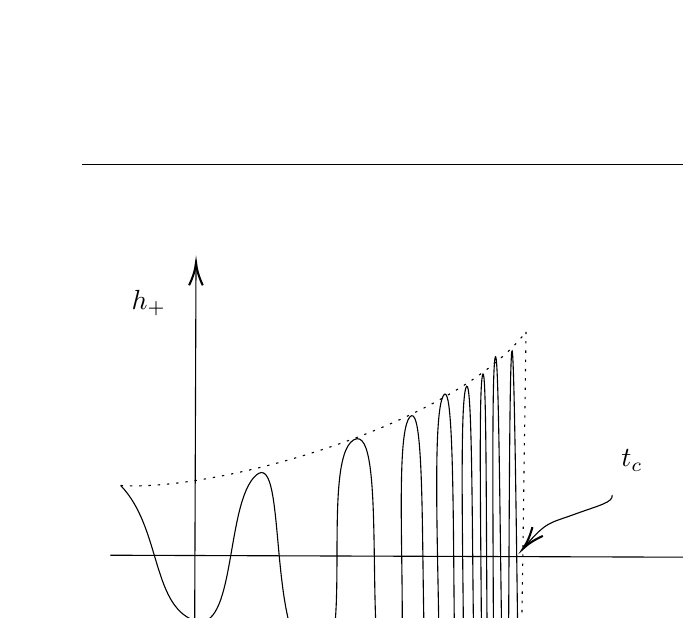
\begin{tikzpicture}[x=0.75pt,y=0.75pt,yscale=-1,xscale=1]
%uncomment if require: \path (0,300); %set diagram left start at 0, and has height of 300

%Straight Lines [id:da9335453423123925]
\draw    (28,150) -- (317.3,150.99) ;
\draw [shift={(319.3,151)}, rotate = 180.2] [color={rgb, 255:red, 0; green, 0; blue, 0 }  ][line width=0.75]    (10.93,-3.29) .. controls (6.95,-1.4) and (3.31,-0.3) .. (0,0) .. controls (3.31,0.3) and (6.95,1.4) .. (10.93,3.29)   ;
%Straight Lines [id:da0384150897274953]
\draw    (68.3,279) -- (69.29,11) ;
\draw [shift={(69.3,9)}, rotate = 450.21] [color={rgb, 255:red, 0; green, 0; blue, 0 }  ][line width=0.75]    (10.93,-3.29) .. controls (6.95,-1.4) and (3.31,-0.3) .. (0,0) .. controls (3.31,0.3) and (6.95,1.4) .. (10.93,3.29)   ;
%Curve Lines [id:da7934604367229809]
\draw  [dash pattern={on 0.84pt off 2.51pt}]  (33,116.4) .. controls (78.3,119.4) and (192.3,88.4) .. (228.3,42.4) ;
%Curve Lines [id:da34437742667793625]
\draw  [dash pattern={on 0.84pt off 2.51pt}]  (34,183.4) .. controls (70.3,170.4) and (181.3,223.4) .. (225.3,251.4) ;
%Straight Lines [id:da09852976233409261]
\draw  [dash pattern={on 0.84pt off 2.51pt}]  (228.3,42.4) -- (225.3,251.4) ;
%Curve Lines [id:da31742712262563155]
\draw    (33,116.4) .. controls (52.3,136.4) and (47.92,173.69) .. (68.3,181.4) .. controls (88.68,189.11) and (83.3,124.4) .. (98.3,111.4) .. controls (113.3,98.4) and (103.3,192.06) .. (125.3,201.4) .. controls (147.3,210.74) and (128.37,104.17) .. (145.3,94.4) .. controls (162.23,84.63) and (149.03,207.03) .. (162.3,217.4) .. controls (175.57,227.77) and (162.24,95.06) .. (172.3,83.4) .. controls (182.36,71.74) and (175.29,218.4) .. (183.3,228.4) .. controls (191.31,238.4) and (180.42,89.71) .. (188.3,73.4) .. controls (196.18,57.09) and (191.39,229.44) .. (196.3,238.4) .. controls (201.21,247.36) and (194.65,83.75) .. (199.3,69.4) .. controls (203.95,55.05) and (201.38,231.32) .. (205.3,242.4) .. controls (209.22,253.48) and (204.26,76.83) .. (207.3,63.4) .. controls (210.34,49.97) and (208.23,234.82) .. (211.3,248.4) .. controls (214.37,261.98) and (210.74,73.03) .. (213.3,55.4) .. controls (215.86,37.77) and (216.03,232.94) .. (218.3,249.4) .. controls (220.57,265.86) and (219.59,78.12) .. (221.3,53.4) .. controls (223.01,28.68) and (224.8,259.9) .. (225.3,251.4) ;
%Curve Lines [id:da08576222941381051]
\draw    (269.8,120.9) .. controls (270.42,124.63) and (263.36,125.97) .. (251.3,130.4) .. controls (239.66,134.68) and (238.38,133.49) .. (227.97,145.54) ;
\draw [shift={(226.8,146.9)}, rotate = 310.43] [color={rgb, 255:red, 0; green, 0; blue, 0 }  ][line width=0.75]    (10.93,-3.29) .. controls (6.95,-1.4) and (3.31,-0.3) .. (0,0) .. controls (3.31,0.3) and (6.95,1.4) .. (10.93,3.29)   ;

% Text Node
\draw (323,161) node [anchor=north west][inner sep=0.75pt]   [align=left] {$\displaystyle t$};
% Text Node
\draw (37,21) node [anchor=north west][inner sep=0.75pt]   [align=left] {$\displaystyle h_{+}$};
% Text Node
\draw (273,98) node [anchor=north west][inner sep=0.75pt]   [align=left] {$\displaystyle t_{c}$};


\end{tikzpicture}


        \caption{ The binary oscillates slowly first, but the oscillation gets faster, wavelength gets shorter and shorter until $t_c$. }
            \end{center}
    \end{figure}


If we draw on of the polarization components of the binary we know it is going to be oscillatory. The binaries oscillate at approximately constant frequency at any given moment of time. That frequency increases till time $t_c$ when everything formally becomes infinite. However, before $t_c$ objects will collide and terminate the process.

If we plot the frequency vs time the frequency will sweep upward and there will be some merger which cuts of the approximation we can make with the tools we have got so far. This are known as "chirps", as sounds which sweep upwards in frequency over time are known as "chirps".



    \begin{figure} [H]
        \begin{center}


\tikzset{every picture/.style={line width=0.75pt}} %set default line width to 0.75pt

\begin{tikzpicture}[x=0.75pt,y=0.75pt,yscale=-1,xscale=1]
%uncomment if require: \path (0,300); %set diagram left start at 0, and has height of 300

%Straight Lines [id:da12827743701411753]
\draw    (88.3,299) -- (89.29,31) ;
\draw [shift={(89.3,29)}, rotate = 450.21] [color={rgb, 255:red, 0; green, 0; blue, 0 }  ][line width=0.75]    (10.93,-3.29) .. controls (6.95,-1.4) and (3.31,-0.3) .. (0,0) .. controls (3.31,0.3) and (6.95,1.4) .. (10.93,3.29)   ;
%Straight Lines [id:da3691885633886325]
\draw    (48,170) -- (337.3,170.99) ;
\draw [shift={(339.3,171)}, rotate = 180.2] [color={rgb, 255:red, 0; green, 0; blue, 0 }  ][line width=0.75]    (10.93,-3.29) .. controls (6.95,-1.4) and (3.31,-0.3) .. (0,0) .. controls (3.31,0.3) and (6.95,1.4) .. (10.93,3.29)   ;
%Curve Lines [id:da6882838800224438]
\draw    (61,139.4) .. controls (106.3,142.4) and (220.3,111.4) .. (256.3,65.4) ;
%Shape: Free Drawing [id:dp4946204585626195]
\draw  [color={rgb, 255:red, 0; green, 0; blue, 0 }  ][line width=3] [line join = round][line cap = round] (257.3,64.2) .. controls (257.3,64.2) and (257.3,64.2) .. (257.3,64.2) ;

% Text Node
\draw (57,41) node [anchor=north west][inner sep=0.75pt]   [align=left] {$\displaystyle f$};
% Text Node
\draw (338,185) node [anchor=north west][inner sep=0.75pt]   [align=left] {$\displaystyle t$};


\end{tikzpicture}



        \caption{ As for the sounds which sweep upwards in frequency over time are known as "chirps", we use the same terminology for GWs. }
            \end{center}
    \end{figure}

We often liken gravitational signals to audio signals, since for BHs which are several times massive than the sun, oscillations  are are in the audio band (100-1000 Hz) when they are the strongest. Thus, if we ever record the GW we can actually record as a sound file and listen to it. 

It turns out that the frequency is the function of the time and of a particular combination of masses which is called the chirp mass.
\begin{align}
\Omega = \Omega(t,\mathcal{M}_c)
\end{align}

where $\mathcal{M}_c$ is the chirp mass 
\begin{align}
\mathcal{M}_c = \Bigg(\frac{\mu}{m}\Bigg)^{3/5}m = \frac{(m_1m_2)^{3/5}}{(m_1+m_2)^{1/5}}
\end{align}

We recall
\begin{align}
f_{GW} = 2f_{orb} = \frac{\Omega}{\pi}
\end{align}

To find $\mathcal{M}_c$ it is enough to find $f_{GW}$ and $\dot{f}_{GW}$ from the phase of the oscillation. Unfortunately this alone does not give us masses $m_1,m_2$ individually. From higher orders in approximation theory we can find the mass ratio:
\begin{align}
q = \frac{m_2}{m_1}
\end{align}

and if we combine this information with the chirp mass, they will give us separate estimate of each mass, but the measurement of $q$ is much worse than the measurement of $\mathcal{M}_c$.
The amplitude of GWs depend on $\Omega(t), \mathcal{M}_c,D$. From this we can get the distance to the radiating object. However, we need to measure both polarizations to know the inclination of the binary. If the binary is orbiting in the $xy$ plane, then the signal (that consists of two polarizations) seen by an observer (Figure 5) depends on $\theta$ and $\phi$, but $\phi$ is only in the overall phase and does not enter in the amplitude. If we measure both polarizations $h_+$ and $h_\times$, by the ratio we can measure the inclination we are at. Therefore, we can measure the distance $D$. 


    \begin{figure} [H]
        \begin{center}



\tikzset{every picture/.style={line width=0.75pt}} %set default line width to 0.75pt

\begin{tikzpicture}[x=0.75pt,y=0.75pt,yscale=-1,xscale=1]
%uncomment if require: \path (0,300); %set diagram left start at 0, and has height of 300

%Straight Lines [id:da9362063425675453]
\draw    (100.3,237) -- (101.29,38) ;
\draw [shift={(101.3,36)}, rotate = 450.29] [color={rgb, 255:red, 0; green, 0; blue, 0 }  ][line width=0.75]    (10.93,-3.29) .. controls (6.95,-1.4) and (3.31,-0.3) .. (0,0) .. controls (3.31,0.3) and (6.95,1.4) .. (10.93,3.29)   ;
%Straight Lines [id:da7949314481364078]
\draw    (10,153) -- (307.3,153.99) ;
\draw [shift={(309.3,154)}, rotate = 180.19] [color={rgb, 255:red, 0; green, 0; blue, 0 }  ][line width=0.75]    (10.93,-3.29) .. controls (6.95,-1.4) and (3.31,-0.3) .. (0,0) .. controls (3.31,0.3) and (6.95,1.4) .. (10.93,3.29)   ;
%Straight Lines [id:da21742408866100638]
\draw    (68,190) -- (160.96,86.49) ;
\draw [shift={(162.3,85)}, rotate = 491.93] [color={rgb, 255:red, 0; green, 0; blue, 0 }  ][line width=0.75]    (10.93,-3.29) .. controls (6.95,-1.4) and (3.31,-0.3) .. (0,0) .. controls (3.31,0.3) and (6.95,1.4) .. (10.93,3.29)   ;
%Straight Lines [id:da2746501081559207]
\draw    (101,153) -- (372.4,61.64) ;
\draw [shift={(374.3,61)}, rotate = 521.4] [color={rgb, 255:red, 0; green, 0; blue, 0 }  ][line width=0.75]    (10.93,-3.29) .. controls (6.95,-1.4) and (3.31,-0.3) .. (0,0) .. controls (3.31,0.3) and (6.95,1.4) .. (10.93,3.29)   ;
%Straight Lines [id:da957406660763626]
\draw    (380,34) -- (423.3,45) ;
%Straight Lines [id:da7663905787557306]
\draw    (394.3,69) -- (423.3,45) ;
%Curve Lines [id:da8650821717889221]
\draw    (389.3,35) .. controls (390.3,36) and (381.3,57) .. (400.3,63) ;
%Curve Lines [id:da34677119565528214]
\draw    (102.3,92) .. controls (109.3,90) and (154.3,103) .. (159.3,131) ;
%Curve Lines [id:da5433303924896837]
\draw    (358.3,37) .. controls (356.3,48) and (354.3,53) .. (370.3,52) ;
%Curve Lines [id:da020242908128639492]
\draw    (380.3,67) .. controls (381.3,68) and (361.3,77) .. (379.3,89) ;
%Curve Lines [id:da4395640039278106]
\draw    (338.3,45) .. controls (353.3,45) and (351.3,60) .. (343.3,66) ;
%Curve Lines [id:da10248702768388696]
\draw    (349.3,79) .. controls (363.3,82) and (362.3,84) .. (361.3,95) ;
%Shape: Ellipse [id:dp31036805732789663]
\draw   (122.06,148.23) .. controls (122.06,144.55) and (125.51,141.56) .. (129.77,141.56) .. controls (134.03,141.56) and (137.48,144.55) .. (137.48,148.23) .. controls (137.48,151.92) and (134.03,154.91) .. (129.77,154.91) .. controls (125.51,154.91) and (122.06,151.92) .. (122.06,148.23) -- cycle ;
%Shape: Ellipse [id:dp8703196193376608]
\draw   (65.94,158.12) .. controls (65.94,154.43) and (69.39,151.44) .. (73.64,151.44) .. controls (77.9,151.44) and (81.35,154.43) .. (81.35,158.12) .. controls (81.35,161.81) and (77.9,164.8) .. (73.64,164.8) .. controls (69.39,164.8) and (65.94,161.81) .. (65.94,158.12) -- cycle ;
%Curve Lines [id:da5161726575364516]
\draw    (76.11,164.8) .. controls (80.32,169.24) and (94.29,173.09) .. (106.29,166.22) ;
\draw [shift={(107.97,165.17)}, rotate = 506.12] [color={rgb, 255:red, 0; green, 0; blue, 0 }  ][line width=0.75]    (10.93,-3.29) .. controls (6.95,-1.4) and (3.31,-0.3) .. (0,0) .. controls (3.31,0.3) and (6.95,1.4) .. (10.93,3.29)   ;
%Curve Lines [id:da6010154202570615]
\draw    (126.69,141.56) .. controls (115.53,132.66) and (101.86,133.25) .. (93.58,137.95) ;
\draw [shift={(91.93,138.99)}, rotate = 325.02] [color={rgb, 255:red, 0; green, 0; blue, 0 }  ][line width=0.75]    (10.93,-3.29) .. controls (6.95,-1.4) and (3.31,-0.3) .. (0,0) .. controls (3.31,0.3) and (6.95,1.4) .. (10.93,3.29)   ;
%Straight Lines [id:da5528803544409464]
\draw    (55.14,168.81) -- (64.79,176.66) ;
%Straight Lines [id:da9992114210507415]
\draw    (52.06,171.48) -- (61.71,179.33) ;
%Straight Lines [id:da3373332191813576]
\draw    (57.3,132.21) -- (50.3,139.79) ;
%Straight Lines [id:da7662189517606179]
\draw    (60.69,134.61) -- (53.69,142.2) ;
%Straight Lines [id:da10513252419362495]
\draw    (139.95,131.14) -- (149.6,138.99) ;
%Straight Lines [id:da09756252458952819]
\draw    (143.65,129) -- (153.3,136.85) ;
%Straight Lines [id:da7951235517923152]
\draw    (145.81,170.68) -- (138.81,178.26) ;
%Straight Lines [id:da050189241617247804]
\draw    (149.51,172.81) -- (142.51,180.4) ;

% Text Node
\draw (130,65) node [anchor=north west][inner sep=0.75pt]   [align=left] {$\displaystyle \theta $};
% Text Node
\draw (313,165) node [anchor=north west][inner sep=0.75pt]   [align=left] {$\displaystyle x$};
% Text Node
\draw (183,64) node [anchor=north west][inner sep=0.75pt]   [align=left] {$\displaystyle y$};
% Text Node
\draw (78,15) node [anchor=north west][inner sep=0.75pt]   [align=left] {$\displaystyle z$};


\end{tikzpicture}


        \caption{ If the binary is orbiting in xy and the amplitude of the radiated GW depends on the angle $\theta$ between the observer and the z axis.}
            \end{center}
    \end{figure}


In reality we do not measure both polarizations due to the sensitivity of the detectors which is called a response function, which is how sensitive you are to GWs coming from different angles.


    \begin{figure} [H]
        \begin{center}



\tikzset{every picture/.style={line width=0.75pt}} %set default line width to 0.75pt

\begin{tikzpicture}[x=0.75pt,y=0.75pt,yscale=-1,xscale=1]
%uncomment if require: \path (0,300); %set diagram left start at 0, and has height of 300

%Curve Lines [id:da08903033563260188]
\draw    (98,110) .. controls (108.39,89.54) and (149.95,74.45) .. (199.33,68.48) .. controls (270.18,59.92) and (357.12,70.13) .. (391.3,110.2) ;
%Straight Lines [id:da5691209566202127]
\draw    (210.3,87.2) -- (203,162) ;
%Straight Lines [id:da1155876869421748]
\draw    (195.65,86.1) -- (224.95,88.3) ;
%Straight Lines [id:da5653215815978823]
\draw    (281.3,168.2) -- (203,162) ;
%Straight Lines [id:da46807102777249376]
\draw    (282.47,156.15) -- (280.12,180.25) ;
%Straight Lines [id:da5620984866836409]
\draw  [dash pattern={on 0.84pt off 2.51pt}]  (61.3,105.2) -- (203,162) ;

% Text Node
\draw (172,112) node [anchor=north west][inner sep=0.75pt]   [align=left] {$\displaystyle L_{1}$};
% Text Node
\draw (241,176) node [anchor=north west][inner sep=0.75pt]   [align=left] {$\displaystyle L_{2}$};
% Text Node
\draw (221,100) node [anchor=north west][inner sep=0.75pt]   [align=left] {$\displaystyle y$};
% Text Node
\draw (252,136) node [anchor=north west][inner sep=0.75pt]   [align=left] {$\displaystyle x$};


\end{tikzpicture}


        \caption{ The interferometer measures the relative distance $L_1-L_2$. }
            \end{center}
    \end{figure}

On the earth you build an interferometer with the L shape. The goal of this interferometer is to measure the relative distance between $L_1$ and $L_2$ (Figure 6),but it only detects GWs which have + polarization, since x polarization does not move distances along either these two lengths. This detector has a sensitivity pattern and it has got a response function to $h_+$ and a response function to  $h_\times$.
Furthermore, if the wave comes in relative to the ground, unless you know where it came from, you do not know how much your amplitude  is degraded by the particular angle that the GWS are coming in. The binary could have been in the other direction (Figure 7) which might have had a different response function to your detector.


    \begin{figure} [H]
        \begin{center}


\tikzset{every picture/.style={line width=0.75pt}} %set default line width to 0.75pt

\begin{tikzpicture}[x=0.75pt,y=0.75pt,yscale=-1,xscale=1]
%uncomment if require: \path (0,300); %set diagram left start at 0, and has height of 300

%Straight Lines [id:da865815865763065]
\draw    (81,114) -- (211.3,114.4) ;
%Straight Lines [id:da6110519257096092]
\draw    (422,109) -- (552.3,109.4) ;
%Straight Lines [id:da3808353035636727]
\draw    (285.3,286) -- (286.29,87) ;
\draw [shift={(286.3,85)}, rotate = 450.29] [color={rgb, 255:red, 0; green, 0; blue, 0 }  ][line width=0.75]    (10.93,-3.29) .. controls (6.95,-1.4) and (3.31,-0.3) .. (0,0) .. controls (3.31,0.3) and (6.95,1.4) .. (10.93,3.29)   ;
%Straight Lines [id:da07350569310066746]
\draw    (195,202) -- (492.3,202.99) ;
\draw [shift={(494.3,203)}, rotate = 180.19] [color={rgb, 255:red, 0; green, 0; blue, 0 }  ][line width=0.75]    (10.93,-3.29) .. controls (6.95,-1.4) and (3.31,-0.3) .. (0,0) .. controls (3.31,0.3) and (6.95,1.4) .. (10.93,3.29)   ;
%Straight Lines [id:da7948212292221113]
\draw    (260.3,247.4) -- (324.3,137.13) ;
\draw [shift={(325.3,135.4)}, rotate = 480.13] [color={rgb, 255:red, 0; green, 0; blue, 0 }  ][line width=0.75]    (10.93,-3.29) .. controls (6.95,-1.4) and (3.31,-0.3) .. (0,0) .. controls (3.31,0.3) and (6.95,1.4) .. (10.93,3.29)   ;
%Straight Lines [id:da17020411077459507]
\draw    (365,102) -- (393.3,127.4) ;
%Straight Lines [id:da37821966901482607]
\draw    (403.3,92.4) -- (285.3,203.4) ;
%Straight Lines [id:da48022323376048304]
\draw    (356,111) -- (384.3,136.4) ;
%Straight Lines [id:da44970445129309744]
\draw    (374,94) -- (402.3,119.4) ;
%Straight Lines [id:da971007183399994]
\draw    (440.3,56.4) -- (425.96,70.14) -- (397.59,97.32) ;
\draw [shift={(396.15,98.7)}, rotate = 316.23] [color={rgb, 255:red, 0; green, 0; blue, 0 }  ][line width=0.75]    (10.93,-3.29) .. controls (6.95,-1.4) and (3.31,-0.3) .. (0,0) .. controls (3.31,0.3) and (6.95,1.4) .. (10.93,3.29)   ;
%Shape: Ellipse [id:dp8662007622106462]
\draw   (531.06,23.23) .. controls (531.06,19.55) and (534.51,16.56) .. (538.77,16.56) .. controls (543.03,16.56) and (546.48,19.55) .. (546.48,23.23) .. controls (546.48,26.92) and (543.03,29.91) .. (538.77,29.91) .. controls (534.51,29.91) and (531.06,26.92) .. (531.06,23.23) -- cycle ;
%Shape: Ellipse [id:dp8948551127382074]
\draw   (474.94,33.12) .. controls (474.94,29.43) and (478.39,26.44) .. (482.64,26.44) .. controls (486.9,26.44) and (490.35,29.43) .. (490.35,33.12) .. controls (490.35,36.81) and (486.9,39.8) .. (482.64,39.8) .. controls (478.39,39.8) and (474.94,36.81) .. (474.94,33.12) -- cycle ;
%Curve Lines [id:da21963501002835972]
\draw    (485.11,39.8) .. controls (489.32,44.24) and (503.29,48.09) .. (515.29,41.22) ;
\draw [shift={(516.97,40.17)}, rotate = 506.12] [color={rgb, 255:red, 0; green, 0; blue, 0 }  ][line width=0.75]    (10.93,-3.29) .. controls (6.95,-1.4) and (3.31,-0.3) .. (0,0) .. controls (3.31,0.3) and (6.95,1.4) .. (10.93,3.29)   ;
%Curve Lines [id:da9456993561289924]
\draw    (535.69,16.56) .. controls (524.53,7.66) and (510.86,8.25) .. (502.58,12.95) ;
\draw [shift={(500.93,13.99)}, rotate = 325.02] [color={rgb, 255:red, 0; green, 0; blue, 0 }  ][line width=0.75]    (10.93,-3.29) .. controls (6.95,-1.4) and (3.31,-0.3) .. (0,0) .. controls (3.31,0.3) and (6.95,1.4) .. (10.93,3.29)   ;
%Straight Lines [id:da4264596286507911]
\draw    (464.14,43.81) -- (473.79,51.66) ;
%Straight Lines [id:da056961842638754145]
\draw    (461.06,46.48) -- (470.71,54.33) ;
%Straight Lines [id:da8910123741373661]
\draw    (466.3,7.21) -- (459.3,14.79) ;
%Straight Lines [id:da5838797688288626]
\draw    (469.69,9.61) -- (462.69,17.2) ;
%Straight Lines [id:da7421622037039197]
\draw    (548.95,6.14) -- (558.6,13.99) ;
%Straight Lines [id:da2473940960232932]
\draw    (552.65,4) -- (562.3,11.85) ;
%Straight Lines [id:da006870569387358971]
\draw    (554.81,45.68) -- (547.81,53.26) ;
%Straight Lines [id:da4316982403773064]
\draw    (558.51,47.81) -- (551.51,55.4) ;
%Straight Lines [id:da45057377864073045]
\draw    (157.3,131.4) -- (285.3,203.4) ;
%Straight Lines [id:da3358004770945615]
\draw    (217.3,144.4) -- (192.3,175.4) ;
%Straight Lines [id:da2968790611555039]
\draw    (206.3,137.4) -- (186.39,162.09) -- (181.3,168.4) ;
%Straight Lines [id:da4883499578189827]
\draw    (228.3,151.4) -- (203.3,182.4) ;




\end{tikzpicture}


        \caption{ If we have just one interferometer we do not know the direction of the incoming GWs - the amplitude is degraded by the inclination angle. }
            \end{center}
    \end{figure}
    
That is why having multiple detectors have advantages. In that case you can triangulate where these objects are in the sky. Each detector in general is blind to one polarization. Therefore, multiple detectors enable us to simultaneously measure both polarizations in addition to the direciton, so we can get the distance $D$ to these sources.



\end{document}
